\itemhead{习题4.1 · 第8题（教材p.104）}{XJ-B1-C04-HW-P104-Y1494}
\label{XJ-B1-C04-HW-P104-Y1494}
{\footnotesize 湘教版教材p.104 / PDF第111页 / 习题4.1 / 第8题}
\field{原题}{已知幂函数 $f(x)=x^\alpha$ 的图象经过点 $\left(8,\dfrac12\right)$，求函数的表达式，并画出它的图象的草图，讨论它的奇偶性和单调性。}
\field{参考答案}{$f(x)=x^{-1/3}=1/\sqrt[3]x$，定义域 $\mathbb R\setminus\{0\}$，奇函数；在 $(-\infty,0)$、$(0,+\infty)$ 分别递减，无增区间；图象在第一、三象限，经过 $(1,1),(-1,-1)$。}
\begin{center}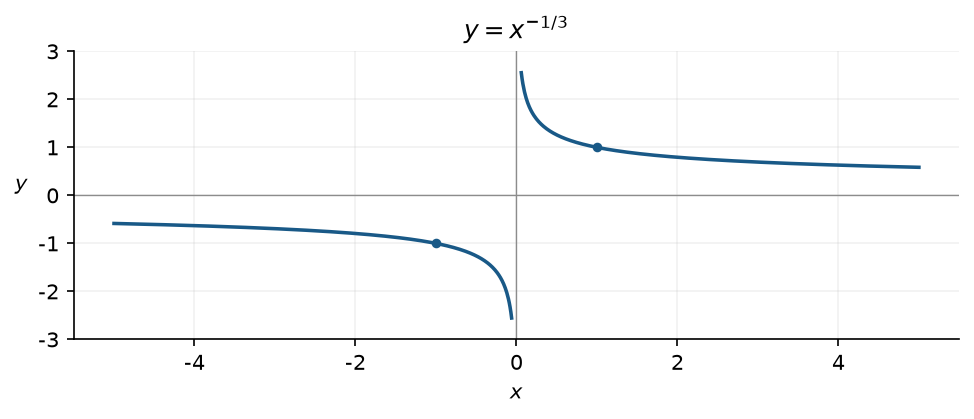
\includegraphics[width=.84\linewidth,height=.38\textheight,keepaspectratio]{figures/C04-HW104-8.png}\end{center}
{\small \field{关联知识}{P03 幂函数的概念、图象与性质（教材帮p.125、126、127 / PDF134、135、136）；F08 奇偶性、对称与函数性质应用（教材帮p.113、114、115 / PDF122、123、124）；F05 单调性定义、证明与参数（教材帮p.97、98、100 / PDF106、107、109）}
\field{方法与易错点}{设 $f(x)=x^\alpha$，用已知点求指数，再查该指数的定义域、奇偶性和各单调区间。 易错：把 $3x^2$ 当标准幂函数；将第一象限性质直接用于负半轴；分数负指数遗漏0禁点。}
\field{答案依据}{答案册相关题组：PDF第31页（册内页30）；按当前题库原题逐项重算，不按旧版题号机械对套。}}
